\documentclass[serif,mathserif]{beamer}
\usepackage{etex}
\usepackage{amsmath, amsfonts, epsfig, xspace}
\usepackage{algorithm,algorithmic}
\usepackage{pstricks,pst-node}
\usepackage{multimedia}
\usepackage[normal,tight,center]{subfigure}
\setlength{\subfigcapskip}{-.5em}
\usepackage{beamerthemesplit}
\usetheme{lankton-keynote}
\usepackage{graphicx,color}
% remove caption of figure
\usepackage[labelformat=empty]{caption}

\usepackage[none]{hyphenat} % hyphenation is ugly in slides
\usepackage{parskip}

\usepackage{relsize} % \smaller to change size

\usepackage{tikz}
\usetikzlibrary{calc}

\usetikzlibrary{arrows}

\newcommand{\TikzDraw}[2][]{
  \begin{tikzpicture}[overlay, remember picture, shift={(current page.center)}, #1]
    #2
  \end{tikzpicture}
}

\newcommand{\gridlines}{
  \TikzDraw{
    \draw[help lines,xstep=.2,ystep=.2,red!20] (current page.south west) grid (current page.north east);
    \draw[help lines,xstep=1,ystep=1,red] (current page.south west) grid (current page.north east);
    \foreach \x in {-15,-14,...,15} {
      \node [anchor=north, red] at (\x,0) {\tiny \x};
      \node [anchor=east,red] at (0,\x) {\tiny \x};
    }
  }
}

\newcommand{\DrawOnImg}[3][]
{
  \begin{tikzpicture}
    \node[anchor=south west,inner sep=0] (image) at (0,0){
      #2
    };
    \begin{scope}[x={(image.south east)},y={(image.north west)}]
      \ifthenelse{\equal{#1}{grid}}
                 {\draw[color=blue, style=dashed] (0,0) grid[xstep=.1, ystep=.1] (1.0001,1.0001);}
                 {}
                 #3
    \end{scope}
  \end{tikzpicture}
}

\usetikzlibrary{matrix}

\newcommand{\BOLD}[1]{\mathbf{#1}}
\newcommand{\BOLDG}[1]{\boldsymbol{#1}}
\newcommand{\PDIF}[2]{\frac{\partial #1}{\partial #2}}
\newcommand{\TODO}[1]{\textcolor{red}{#1}}
\newcommand{\TODOB}[1]{\textcolor{blue}{#1}}
\newcommand{\TODOG}[1]{\textcolor{green!50!black}{#1}}
\newcommand{\argmin}{\operatornamewithlimits{arg\min}}
\DeclareMathOperator{\tr}{tr}
\DeclareMathOperator{\cond}{cond}
\DeclareMathOperator{\ST}{s.t.}
\DeclareMathOperator{\diag}{diag}

\author[Jiong Chen]{Jiong Chen}

\title[\hspace{2em}\insertframenumber/\inserttotalframenumber]{Microstructures to Control Elasticity in 3D Printing}

\date{April 21, 2017}

% \institute{Zhejiang University}

\begin{document}

\maketitle

\begin{frame}
  \frametitle{Motivation}
  \begin{itemize}
  \item A simple question
    \begin{itemize}
    \item[-] How to fabricate deformable objects with spatially varying elasticity using a single, relatively
      stiff printer material?
    \end{itemize}
  \end{itemize}
  \TikzDraw {
    \node at (-2.9, -2) {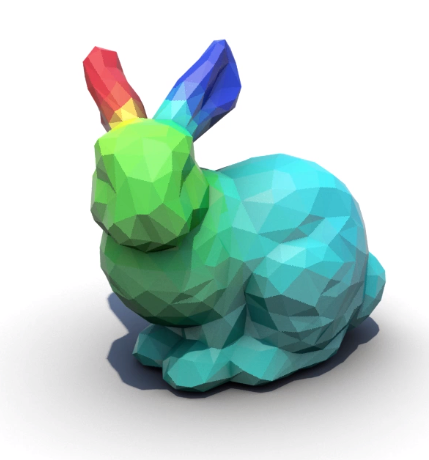
\includegraphics[scale=0.2]{img/bunny}};
    \node at (0.1, -2.17) {
\includegraphics[scale=0.19]{img/teddy}};
    \node at (3.1, -2.1) {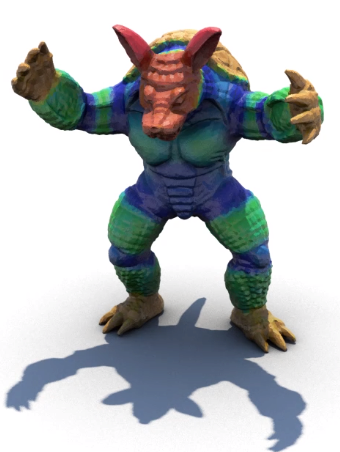
\includegraphics[scale=0.2]{img/armadillo}};
  }
\end{frame}

\begin{frame}
  \frametitle{Overview}
  \begin{itemize}
  \item Metamaterial
  \item Material space
  \item Synthesis
  \end{itemize}
  \TikzDraw {
    \visible<2-> {\node at (1.2, 0.6) {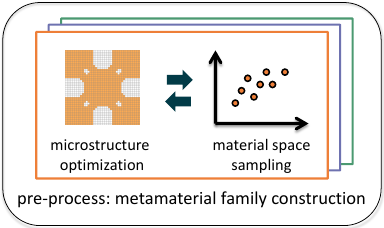
\includegraphics[scale=0.3]{img/preprocess}};}
    \visible<3> {\node at (0, -2) {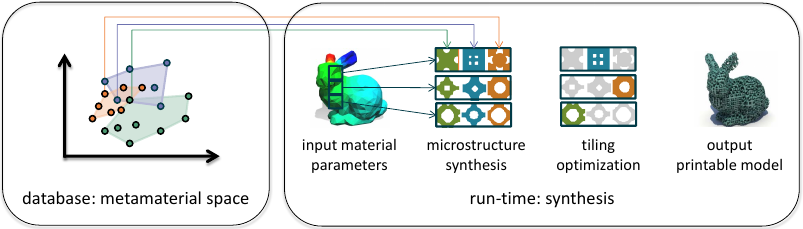
\includegraphics[scale=0.3]{img/runtime}};}
    \visible<2> {\draw[red, thick] (-5.2, 0.2) rectangle (-1.8, 1.6);}
    \visible<3> {\draw[red, thick] (-5.2, -0.5) rectangle (-2.5, 0.1);}
  }
%  \gridlines
\end{frame}

\begin{frame} 
  \TikzDraw {
    \node at (0, 0.5) {\Huge{Preprocessing}};
  }
\end{frame}

\begin{frame}
  \frametitle{Metamaterial}
  \begin{itemize}
  \item Microstructure generation
    \begin{figure}
      \begin{tikzpicture}[every node/.style={minimum size=.5cm-\pgflinewidth, outer sep=0pt}]
        \visible<1-> {\draw[step=0.5cm,color=black] (-1,-1) grid (1,1);}
        \visible<2-> {
          \node[fill=black] at (-0.75,+0.75) {};
          \node[fill=black] at (-0.25,+0.25) {};
          \node[fill=black] at (+0.25,+0.25) {};
          \node[fill=black] at (+0.75,+0.75) {};
          \node[fill=black] at (-0.25,-0.25) {};
          \node[fill=black] at (+0.25,-0.25) {};
          \node[fill=black] at (-0.75,-0.75) {};
          \node[fill=black] at (+0.75,-0.75) {};          
        }
      \end{tikzpicture}
    \end{figure}
    \pause
    \pause
  \item For each voxel
    \begin{equation*}
      \BOLD{C}_i = \BOLDG{\alpha}_i\BOLD{C}_{base}
    \end{equation*}
    \pause
  \item Problem formulation
    \begin{equation*}
      \boxed{
        \begin{split}
        &\min_{\BOLDG{\alpha}} \|\BOLD{C}(\BOLD{p}_{goal})-\mathbb{C}(\BOLD{h}(\BOLDG{\alpha}))\|_F^2 + R\\
        &\ST\quad \alpha_{min} \le \BOLDG{\alpha}_i \le 1, \quad\quad 1 \le i \le m
        \end{split}
        }
    \end{equation*}
  \end{itemize}
\end{frame}

\begin{frame}
  \frametitle{Metamaterial}
  \begin{itemize}
  \item Regularization
    \begin{itemize}
    \item[-] Enforcing integer values
      \begin{equation*}
        R_{int} = \sum_{i=1}^m (\BOLDG{\alpha}_i-\alpha_{min})(1-\BOLDG{\alpha}_i)
      \end{equation*}
      \pause
    \item[-] Smoothness
      \begin{equation*}
        R_s = \sum_{i, j} (\BOLDG{\alpha}_{i-1, j}+\BOLDG{\alpha}_{i+1, j}
        +\BOLDG{\alpha}_{i, j-1}+\BOLDG{\alpha}_{i, j+1}-4\BOLDG{\alpha}_{i, j})^2
      \end{equation*}
      \pause
    \item[-] Checkerboard patterns
      \begin{equation*}
        \begin{split}
        R_{cb}= \sum_{i, j} &(1-\BOLDG{\alpha}_{i, j})(\BOLDG{\alpha}_{i+1, j}-\BOLDG{\alpha}_{min})\\
        &(\BOLDG{\alpha}_{i, j+1}-\BOLDG{\alpha}_{min})(1-\BOLDG{\alpha}_{i+1, j+1}) \\
        +&(1-\BOLDG{\alpha}_{i+1, j})(\BOLDG{\alpha}_{i, j}-\BOLDG{\alpha}_{min})\\
        &(\BOLDG{\alpha}_{i+1, j+1}-\BOLDG{\alpha}_{min})(1-\BOLDG{\alpha}_{i, j+1})
        \end{split}
      \end{equation*}
    \end{itemize}
  \end{itemize}
  \visible<3-> {
    \begin{tikzpicture}[overlay, remember picture, shift={(current page.center)}, every node/.style={minimum size=.5cm-\pgflinewidth, outer sep=0pt}]
      \draw[step=0.5cm,color=black] (-4,-3) grid (-3, -2);
      \node[fill=black] at (-3.75, -2.75) {};
      \node[fill=black] at (-3.25, -2.25) {};
    \end{tikzpicture}
  }
\end{frame}

\begin{frame}
  \frametitle{Effects of Regularization}
  \begin{itemize}
  \item Integer enforcement
    \begin{figure}
      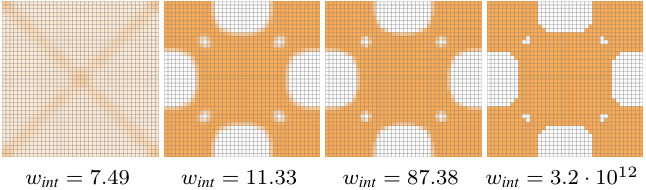
\includegraphics[width=0.5\textwidth]{img/Rint}
    \end{figure}
    \pause
  \item Checkerboard and smoothness
    \begin{figure}
      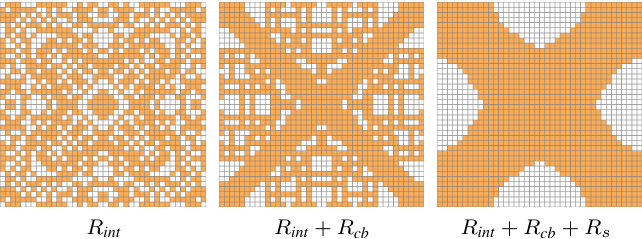
\includegraphics[width=0.5\textwidth]{img/allR}
    \end{figure}
    \pause
  \item Connectivity
    \begin{figure}
      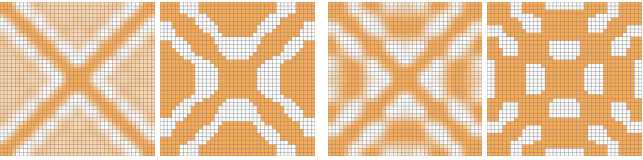
\includegraphics[width=0.5\textwidth]{img/connectivity}
    \end{figure}
  \end{itemize}
\end{frame}

\begin{frame}
  \frametitle{Material Space}
  \begin{itemize}
  \item Microstructure representation
    \begin{itemize}
    \item Geometry: convert voxel to signed distance field in $[0, 1]^d$
      \begin{figure}
        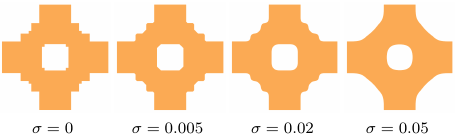
\includegraphics[width=0.5\textwidth]{img/gaussian}
      \end{figure}
      \pause
    \item Representative Material parameters (less DoFs)
      \begin{equation*}
        \begin{split}
        &\min_p \|\BOLD{C}(\BOLD{p})-\hat{\BOLD{C}}\|_F^2 \\
        &\ST\quad p_i^{min} \le \BOLD{p}_i \le p_i^{max}
        \end{split}
      \end{equation*}
    \end{itemize}
  \end{itemize}
\end{frame}

\begin{frame}
  \frametitle{Material Space}
  \begin{itemize}
  \item Material families
    \begin{figure}
      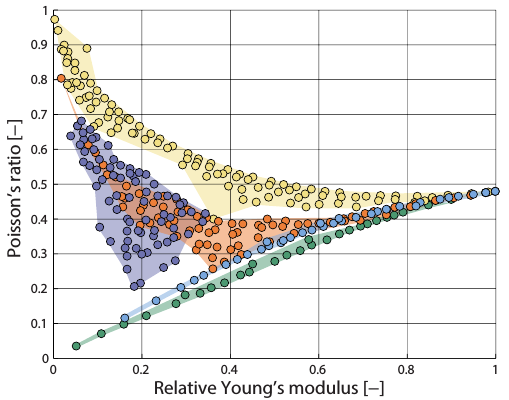
\includegraphics[width=0.5\textwidth]{img/mtrfamily}
    \end{figure}
    \visible<4-> {
    \item Interpolation
      \begin{figure}
        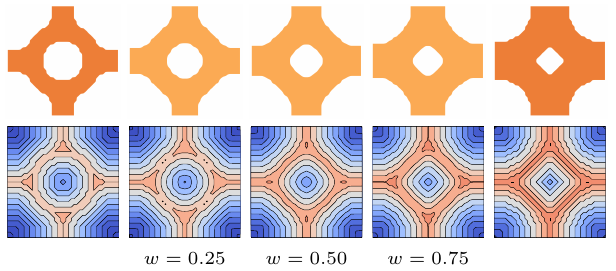
\includegraphics[width=0.4\textwidth]{img/mtrinterp}
      \end{figure}
    }
  \end{itemize}
  \TikzDraw {
    \visible<2-3> {
      \node at (0.4, 0) {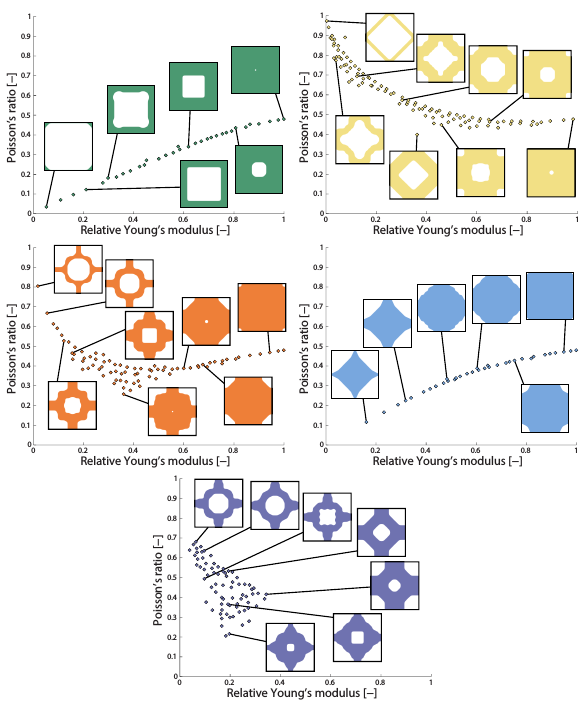
\includegraphics[width=0.5\textwidth]{img/mtrentity}};
    }
    \visible<3> {
      \node at (0.4, 0) {
\includegraphics[width=0.5\textwidth]{img/brokeninterp}};
    }
  }
\end{frame}

\begin{frame}
  \TikzDraw {
    \node at (0, 0.5) {\Huge{Run-time synthesis}};
  }
\end{frame}

\begin{frame}
  \frametitle{Structure Synthesis}
  \begin{itemize}
    \visible<2-> {
    \item Two issues need to be considered
      \begin{itemize}
      \item Structure-parameter matching
      \item Boundary compatibility
      \item[]
        \begin{figure}
          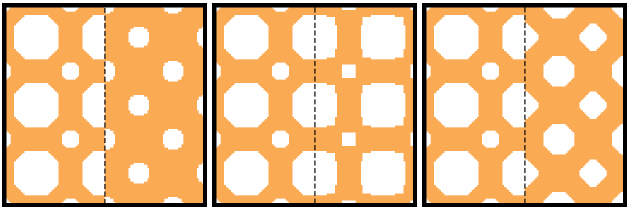
\includegraphics[width=0.5\textwidth]{img/boundary}
        \end{figure}
      \end{itemize}
    }
    \visible<3-> {
    \item Penalties
      \begin{itemize}
      \item Similarity: $T_i^L = e^{d_i}$
      \item Dissimilarity: $T_{i, j}^D = e^{g(i, j)},~g(i, j) = \frac{\int_{\partial \Omega}\|df\|}{\int_{\partial \Omega}\|f\|}$
      \end{itemize}
    }
  \end{itemize}
  \TikzDraw {
    \visible<1> {
      \node at (0, 0) {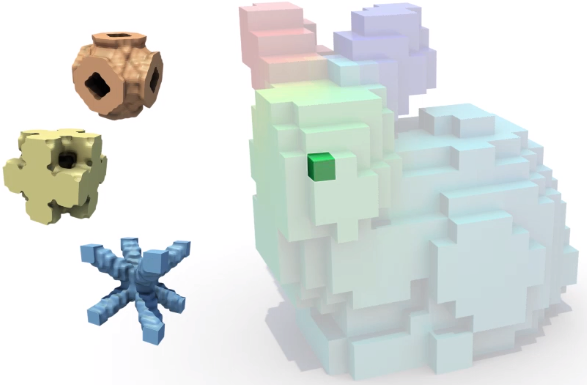
\includegraphics[width=\textwidth]{img/synthesis}};
    }
  }
\end{frame}

\begin{frame}
  \frametitle{Structure Synthesis}
  \begin{itemize}
  \item Solution space
    \begin{figure}
      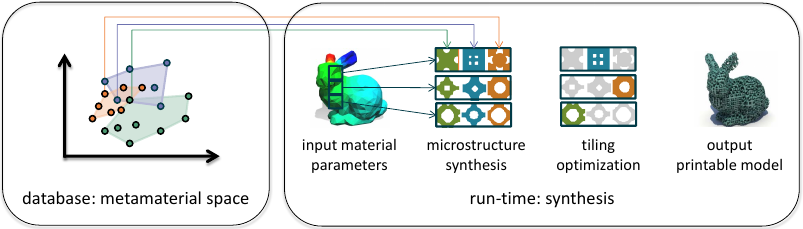
\includegraphics[width=\textwidth]{img/runtime}
    \end{figure}
  \item NP-hard, solved by ADMM.
  \end{itemize}
\end{frame}

\begin{frame}
  \frametitle{Results: 3D Microstructures}
  \begin{figure}
    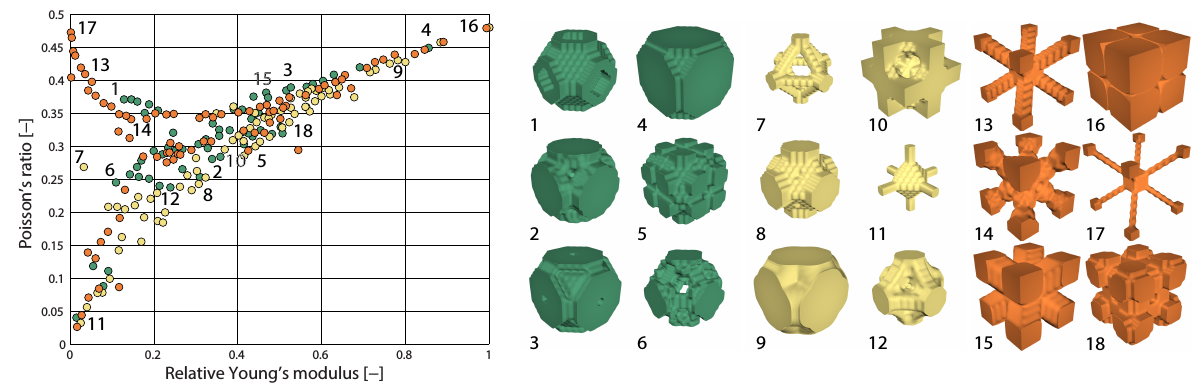
\includegraphics[width=\textwidth]{img/micro3d}
  \end{figure}
\end{frame}

\begin{frame} 
  \TikzDraw {
    \node at (0, 0.5) {\Huge{Thanks!}};
  }
  %\gridlines
\end{frame}


\end{document}
